\documentclass[12pt,a4paper]{univention}
\usepackage[utf8]{inputenc}
\usepackage[T1]{fontenc}
\usepackage{amsmath}
\usepackage{amsfonts}
\usepackage{float}
\usepackage{amssymb}
\usepackage{graphicx}
\author{Julia Bremer}
\setcounter{tocdepth}{2}
\usepackage[T1]{fontenc}
\usepackage{underscore}
\begin{document}

\maketitle{Betriebssysteme Tanenbaum Mitschrift}{Julia Bremer}{}{}
\tableofcontents
\newpage
\section{Kapitel 1 - Einführung}
\subsection{Aufgaben}
\subsubsection{Q: Was sind die zwei Hauptfunktionen eines Betriebssystems?}
A: Die beiden Hauptfunktionen eines Betriebssystem sind Ressourcenverwaltung der Hardware und die Bereitstellung einer einheitlichen Schnittstelle für Programme und Programmiern zu erstellen.
\subsubsection{Q: In Abschnitt 1.4 wurden neun unterschiedliche Betriebssystemarten beschrieben. Geben Sie Anwendungsbeispiele ür jedes dieser Systeme an (eines für jede Betriebssystemart).}
\begin{tabular}{|c|c|}
\hline 
Betriebssystemart & Beispiel \\ 
\hline 
BS für Großrechner\\robust, hochgradig reduntant & Geldautomaten-Systeme \\ 
\hline 
BS für Server\\Zur Bereitstellung von Diensten & Webdienste \\ 
\hline 
BS für Multiprozessorsysteme\\Rechenaufwand wird auf viele Prozessoren verteilt & Simulationen, Wettervorhersagen \\ 
\hline 
BS für PCs\\Anwenderfreundlichkeit & Heimcomputer \\ 
\hline 
BS für Handheld-Computer\\PDA & Smartphones, Tablets \\ 
\hline 
BS für eingebettete Systeme\\Rechensysteme die andere Geräte steuern & Mikrowellen, Autos \\ 
\hline 
BS für Sensorknoten\\Sensornetz & Frühwarnsystem für Waldbrände \\ 
\hline 
Echtzeitbetriebssysteme & industrielle Fertigungssteuerung - Schweißroboter \\ 
\hline 
BS für Smartcards & Kreditkarte \\ 
\hline 
\end{tabular} 
\subsubsection{Q: Worin besteht der Unterschied zwischen Timesharing- und Multiprogrammiersystemen?}
\textbf{Timesharing ist eine Varianz von Multiprogrammierung.}\\
Multiprogrammierung wird genutzt, um Ressourcen optimal(-er) aufteilen zu können. \\
Zuvor konnte die CPU nicht genutzt werden, während sie auf Ein- oder Ausgaben wartete. \\
Um also die Verarbeitung weiterer Aufgaben zu ermöglichen, während die CPU auf Beendigung einer Ein- oder Ausgabe wartet, wurde der Speicher in mehrere Speicherpatitionen aufgeteilt. \\
Die Antwortzeiten hat dies jedoch verlängert, sobald mehrere Leute gleichzeitig Daten verarbeiteten. Kürzere Antwortzeiten waren erwünscht.\\
Daher führte man \textbf{Timesharing} ein.\\
Durch das Timesharing können mehrere Nutzer online Zugang zum System über ein Terminal haben.\\
Mit Multiprogrammierung verfolgt man also das Ziel, die CPU-Zeit effektiv nutzen zu können.\\
Mit Timesharing können nicht nur mehrere Programme die CPU gleichzeitig nutzen, sondern auch viele User, die vielleicht nur kurze Übersetzungen machen wollten.\\ Timesharing benutzt Multiprogrammierung um die CPU für mehrere Nutzer verwendbar zu machen.
\subsubsection{Q: Um Cache-Speicher zu benutzen wird der Arbeitsspeicher in Cache-Lines aufgeteilt, die in der Regel 32 oder 64 Byte lang sind. Eine Cache-Line wird an einem Stück in den Cache geladen. Worin liegt der Vorteil, die gesamte Cache-Line anstelle von einzelnen Bytes oder Wörtern nacheinander zu laden?}
Mithilfe von Cache-Lines können Teile priorisiert werden, also an einem früheren Teil des Caches gespeichert werden. Daten können mit ihrer Blockzahl adressiert werden, sie müssen nicht mit längeren Adresstags angesprochen werden.
Es muss kein Stop-Symbol gespeichert werden, bei einem Cache-Hit muss nicht nach dem Ende des Datensatzes gesucht werden.
\subsubsection{Q: Bei den ersten Computern wurde das Lesen und Schreiben jedes einzelnen Bytes vom Prozessor durchgeführt (d.h., es gab noch keine DMA). Was für Auswirkungen hat das für die Multiprogrammierung?}
DMA = Direct Memory Access\\
Ohne ein DMA-Chip an den der Prozessor die Ein- und Ausleseschritte abgibt, gibt es keine Wartezeit für den Prozessor, die durch Multiprogrammierung gefüllt werden könnte.
\subsubsection{Q: Befehle, die den Zugriff auf Ein-/Ausgabegeräte betreffen, sind in der Regel privilegierte Anweisungen, das heißt, sie können im Kerbmodus ausgeführt werden, aber nicht im Benutzermodus. Geben Sie einen Grund dafür an, warum diese Anweisungen priviligiert sind.}
Im Speicher sind alle für das System wichtigen Informationen gespeichert. Veränderungen dieser könnten das gesamte System zum Absturz bringen.\\Die Speicherverwaltung sollte daher nicht von Anwendern übernommen werden können.\\
Policies, die von Administratoren gesetzt werden, sollen nicht von Anwenderprogrammen umgangen werden können.
\subsubsection{Q: Die Idee, ganze Familien von Rechnern zu bauen wurde in den 1960er Jahren mit dem System/360 von IBM für Großrechner eingeführt. Ist diese Idee heute gestorben oder existiert sie immer noch?}
Diese Idee existiert noch. Intel hat mit i3, i5, i7 CPUs Prozessoren geschaffen, die unter einander verschiedene Schnelligkeiten und Preise haben, aber interoperabel sind.
\subsubsection{Q: Ein Grund für die zurückhaltende Annahme grafischer Benutzungsoberfläcen war, dass die nötige Hardware anfangs noch sehr teuer war. Wie viel Videospeicher braucht man für die Darstellung von 80 Zeichen auf 25 Zeilen Textmodus in Schwarz-Weiß? Und wie viel braucht man für die Darstelung von 1200x900 Bildpunkten mit 24-Bit-Farbtiefe? Was hat der Speicher 1980 gekostet, als ein KB etwa 5 US-Dollar kostete? Und wie viel kostet er heute?}
Die  Menge an Daten die gebraucht wird, ist für eine grafische Darstellung um ein Vielfaches höher.
\begin{align*}
25 \cdot 80 = 2000\\
2000 \cdot \frac{5}{1000} = \underline{\underline{10}}
\end{align*}
Früher hätte der Speicher für Textausgabe 10 US-Dollar gekostet
\begin{align*}
1200 \cdot 900 \cdot 24 = 3.240.000\\
3.240.000 \cdot \frac{5}{1000} =\underline{\underline{16.200}}
\end{align*}
Früher hätte der Speicher für die grafische UI 16.200 US-Dollar gekostet.
Heutzugage wären die Kosten sehr gering. Habe gerade keine Lust Preise anzusehen. Vermutlich Cents.
\subsubsection{Q: Es gibt mehrere Entwurfsziele bei der Entwicklung eines Betriebssystems, z.B. Betriebsmittelausnutzung, Rechtzeitigkeit, Robustheit usw. Geben Sie ein Beispiel für zwei Entwurfsziele, die sich möglicherweise gegenseitig widersprechen.}
TODO
\subsubsection{Q: Worin besteht der Unterschied zwischen Kern- und Benutzermodus? Erläutern Sie, inwiefern die Tatsache, zwei unterschiedliche Modi zu haben, beim Entwurf eines Betriebssystems hilfreich ist}
TODO
\subsubsection{Q: Eine 256-GB-Platte hat 65536 Zylinder mit 255 Sektoren pro Track und 512 Byte pro Sektor. Wie viele Scheiben und Köpfe haben diese Platte? Gehen Sie von einer durchschnittlichen Zylindersuchzeit von 11 ms, einer durchschnittlichen Rotationsverzögerung von 7 ms und Lesegeschwindigkeit von 100 MB/s aus. Berechnen Sie die durchschnittliche Zeit, die benötigt wird, um 400 KB aus einem Sektor zu lesen.}
TODO 
\subsubsection{Q: Welche der folgenden Befehle sollten nur im Kernmodus erlaubt sein?}
a. Sperren aller Unterbrechungen \textbf{X}\\ 
b. Lesen der aktuellen Uhrzeit \\
c. Setzen der aktuellen Uhrzeit \textbf{X}\\
d. Ändern der Speicherzuordnungstabellen \textbf{X}
\subsubsection{Q: Betrachten Sie ein System mit zwei Prozessoren, wobei jeder dieser Prozessoren zwei Threads (Hyperthreading) hat. Nehmen Sie an, dass drei Programme, P0, P1 und P2, mit Laufzeiten von 5, 10 bzw. 20 ms gestartet werden. Wie lange wird es dauern, bis die Ausführung dieser Programme vollständig abgeschlossen sind? Nehmen Sie dazu an, dass alle drei Programme zu 100\% CPU-gebunden sind, sich während der Ausführung nicht gegenseitig blockieren und die einmal zugewiesene CPU nicht getauscht wird.}
TODO
\newpage
\section{Kapitel 2 - Prozesse und Threads}
\subsection{Prozesse}
Eine Plattenanfrage dauert für eine CPU sehr lange.
In der Wartezeit werden deshalb andere Aufgaben ausgeführt (Multiprogrammiersystem.\\
In einem Multiprogrammiersystem wechselt die CPU schnell von Programm zu Programm. Genau genommen wird also nur ein Prozess zur Zeit abgearbeitet(pro Kern / CPU). Aber es können mehrere Prozesse innerhalb von kürzester Zeit bearbeitet werden. Es entsteht die Illusion von Parallelität. Nicht zu vergleichen mit echter parallelität in Multiprozessorsystemen.\\
Zur darstellung dieser Parallelität hat man das \textbf{konzeptionelle Modell von sequenziellen Prozessen} erarbeitet. \\
Ein Prozess ist nichts anderes als ein Programm in der Ausführung inklusive der notwendigen Werte (Befehlszähler, Registerinhalte und Belegungen der Variablen).\\
Das das ständige Wechseln der CPU zwischen den Prozessen kann zu asynchronität führen, da die Geschwindigkeit der Ausführung uneinheitlich ist.\\
Ein Programm ist kein Prozess. Ein Programm ist Plan, der Prozess ist die Ausführung.
\subsubsection{Prozesserzeugung}
\textbf{Es gibt vier Verfahren zur Erzeugung von Prozessen:}\\
a. Inititalisierung von Systemen\\
b. Systemaufruf zum Erzeugen eines Prozesses durch einen anderen Prozess\\
c. Benutzeranfrage, einen neuen Prozess zu erzeugen\\
d. Erzeugung einer Stapelverarbeitung\\\\
Prozesse die im Hintergrund ausgeführt werden, und keinem direkten User zugeordnet werden können heißen \textbf{Daemons}.\\
In Unix gibt es nur einen Systemaufruf zum erzeugen eines neuen Prozesses nämlich \textbf{\textit{fork}}.\\
Dieser Aufruf kopiert den bereits existierenden Prozess und erschafft so einen Kindprozess. Für gewöhnlich führt der Kindprozess dann \textit{execve} aus um sein Speicherabbild zu ändern. In Windows gibt es nur \textit{CreateProcess}.\\
Der Speicher des Kindprozesses ist zwar eine Kopie des Elternprozesses, aber sie haben unterschiedliche Adressräume und benutzen keinen schreibbaren Speicher gleichzeitig.
\subsubsection{Prozessbeendigung}
\textbf{Es gibt vier Verfahren zur Beendigung von Prozessen:}\\
a. Normales Beenden (freiwillig) | exit \\
b. Beenden aufgrund eines Fehlers (freiwillig)\\
c. Beenden aufgrund eines schwerwiegenden Fehlers (unfreiwillig)\\
d. Beenden durch einen anderen Prozess (widerwillig) | kill \\
\subsubsection{Prozesshierarchien}
Wenn ein Kindprozess weitere Prozesse erzeugt, so entsteht eine Prozesshierarchie, oder Prozessfamilie.\\
Beim booten eines UNIX-Systems gibt es eine Prozess namens \textit{init} im Bootimage. Dieser ist die Wurzel des Prozessbaums.\\
In Windows gibt es kein Konzept der Prozesshierarchie.
\subsubsection{Prozesszustände}
\textbf{Es gibt drei Zustände in denen ein Prozess sein kann:}\\
a. rechnend\\
b. rechenbereit\\
c. blockiert\\
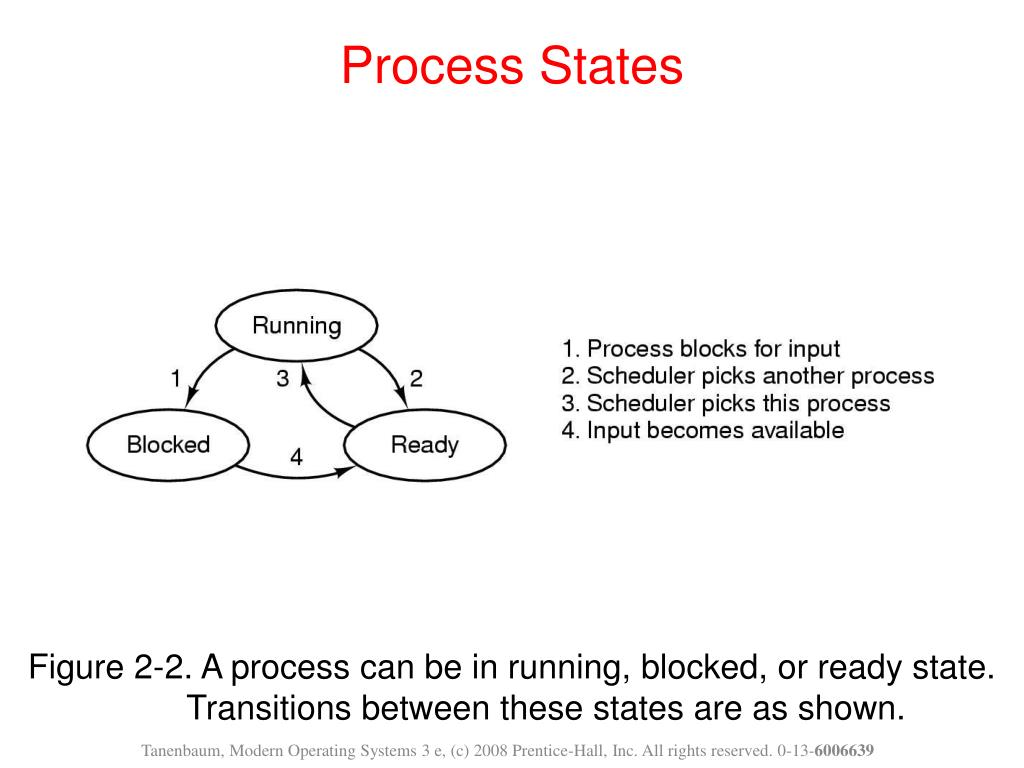
\includegraphics[scale=0.5]{prozesszustaende.jpg}\\
Übergang 2,3 werden vom Prozess-Scheduler ausgeführt, ohne dass der Prozess etwas davon merkt.\\
Das Scheduling muss eine gute Strategie zwischen Effizienz des Systems als Ganzem und Fairness für den einzelnen Prozess finden.\\
Mithilfe eines Festplatteninterrupts trifft das System die Entscheidung einen Prozess anzuhalten und einen anderen Prozess zu starten, der auf diesen interrupt wartete.\\
Das Betriebssystem pflegt eine Prozesstabelle die einen Eintrag pro Prozess hat.\\
Beispiel \textbf{eines} Eintrags in einer Prozesstabelle:\\
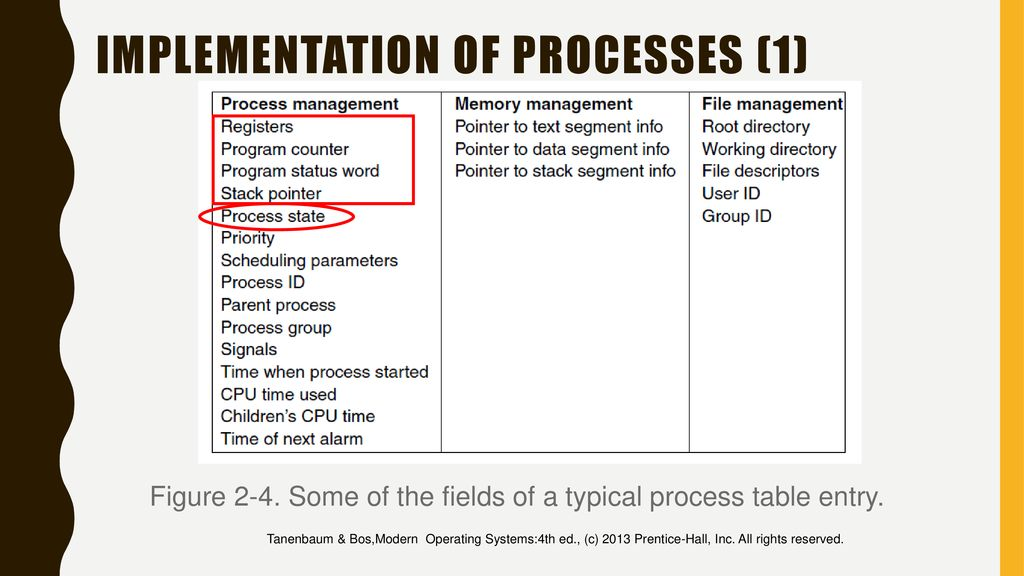
\includegraphics[scale=1]{prozesstabelle.jpg}\\
Um zwischen Prozessen hin- und herzuschalten werden die Adressen der Unterbrechungsroutinen in einem \textbf{Interruptvektor} gespeichert.\\ \textbf{Das Umschalten zwischen Prozessen funktioniert (in etwa) folgendermaßen:}\\
a. Hardware sichert Befehlszähler, Programmstatusantwort und mehr\\
b. Hardware holt neuen Befehlszähler vom Interruptvektor\\
c. Assemblerprozedur speichert Register\\
d. Assemblerprozedur richtet neuen Stack ein\\
e. C-Unterbrechungsroutine läuft (liest und puffert i.d.R. Eingaben)\\
f. Scheduler entscheidet, welcher Prozess als Nächstes läuft\\
g. C-Prozedur kehrt zum Assemblercode zurück\\
h. Assemblerprozedur startet neuen aktuellen Prozess\\\\
Ein Prozess kann tausende Male unterbrochen werden, jedoch soll er sich stets in genau dem selben Zustand wie vor dem Interrupt befinden.
\subsubsection{Modellierung von Multiprogrammierung}
\begin{align*}
&p = \text{Wartezeit der CPU auf Ein-/Ausgaben}\\
&n = \text{Anzahl der Prozesse}\\
&\text{CPU-Ausnutzung} = 1-p^{n}
\end{align*}
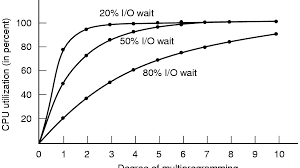
\includegraphics[scale=1]{multiprogramming.png}\\
Interaktive Prozesse, die auf Benutzereingaben warten, haben oft 80 \% oder mehr Wartezeit.
\subsection{Threads}
Prozesse haben alle ihren eigenen Adressraum und einen einzigen Ausführungsfaden (\textit{thread of control}).\\
Manchmal möchte man allerdings noch die Aufgaben innerhalb eines Prozesses parallelisieren. Wenn z.B mehrere Aufgaben gleichzeitig zu erledigen sind.\\
Wenn man also mehrere "Prozesse" haben will, die sich allerdings den gleichen Adressraum teilen, so nutzt man \textbf{Threads.}\\
Ein weiterer Vorteil von Threads ist, dass sie Performanter sind, schneller zu erzeugen und zu zerstören.\\
Dies lohnt sich nur, wenn es nicht nur rechenintensive Threads gibt, sondern auch umfangreiche Ein-/Ausgabeaktivitäten, auf die der Prozess sonst warten müsste.\\
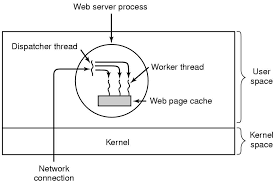
\includegraphics[scale=1]{webserverthread.png}\\
In dieser Abbildung gibt es einen \textbf{Dispatcher} , der ankommende Arbeitsanfragen vom Netzwerk einliest und bei Bedarf   einen \textbf{Worker-Thread} aufweckt und ihm die Anfrage übergibt.\\
Der Dispatcher-Thread ist eine Endlosschleife, die Anfragen entgegennimmt und diese an Worker-Threads weiterleitet. Die Worker-Threads bestehen aus einer Endlosschleife die die Anfragen des Dispatchers annimmt und dann im Cache prüft, ob der angefragte Eintrag vorhanden ist. Dann holt der Worker-Thread holt er dies von der Platte oder aus dem Cache, liefert das Ergebnis und wird dann blockiert.\\
Threads ermöglichen es, das Konzept von sequenziellen Prozessen, die blockerende Systemaufrufe ausführen, beizubehalten und trotzdem Parallelität zu erzielen.
\subsubsection{Das klassische Thread-Modell}
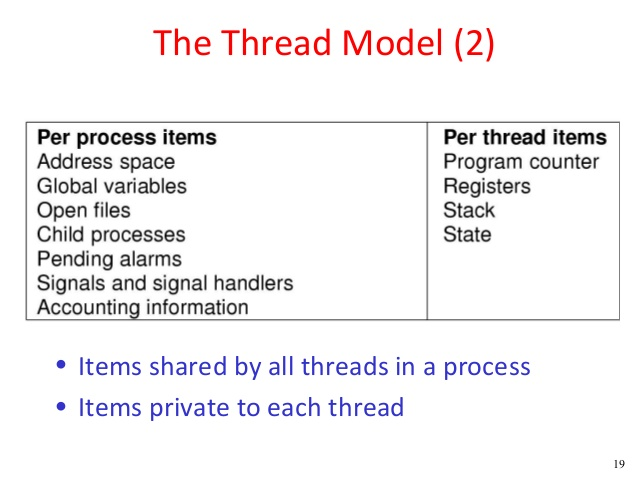
\includegraphics[scale=0.5]{threadmodel.jpg}\\
Threads teilen sich im Gegensatz zu Prozessen ihre Ressourcen.\\
Es ist jedoch wichtig, dass jeder Thread einen eigenen \textbf{Stack} hat.\\
Jeder Stack eines Threads enthält einen Rahmen für die Prozedur mit den lokalen Variablen der Prozedur und der \textbf{Rücksprungsadresse}.\\
Da Threads für gewöhnlich unterschiedliche Prozeduren aufrufen, braucht jeder seine eigene Ablaufhistorie und damit einen eigenen Thread.\\
Ein Prozess der Multithreading benutzt, startet für gewöhnlich als einziger Thread. Mit \textit{thread_create} wird ein neuer Thread gestartet.\\
Mit \textit{thread_exit} kann ein Thread beendet werden. \\
Mit \textit{thread_join} kann ein Thread auf die Beendigung eines anderen Threads warten, bis dahin wird er blockiert.\\
Mit \textit{thread_yield} kann ein Thread freiwillig seine Rechenzeit an einen anderen Thread abgeben. Dies ist wichtig, da es keinen Timeinterrupt wie bei Prozessen gibt. Threads müssen also bewusst ab und an ihre Rechenzeit abgeben.\\\\
Threads bringen jedoch auch Probleme mit sich. Wenn ein Prozess mit meherern Threads geforked wird, sollte dann jeder Kindprozess auch mehrere Threads haben?\\
Wenn nein, kann der Kindprozess möglichweise nicht richtig arbeiten. Wenn ja, und ein Thread im Elternprozess geblockt ist, wird dann auch der Thread im Kindprozess geblockt?\\
Andere Probleme ergeben sich im Speichermanagement. Wenn ein Prozess eine Datei schließt, während ein anderer dies noch liest. Dies kann umgangen werden, ist aber aufwendig und muss bedacht werden.
\subsubsection{POSIX-Threads}
Es gibt einen von der IEEE definierten Standart für die Portierbarkeit von Programmen mit Threads. Das Paket heitß \textbf{Pthread}. Sechs von insgesamt über 60 Funktionsaufrufe sind hier aufgeführt.\\
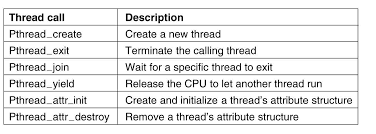
\includegraphics[scale=1]{pthread.png}\\
Threads können auf Anwenderebene oder auf Kernelebene sein. Dazu gibt es verschiedene Vor- und Nachteile.\\\\
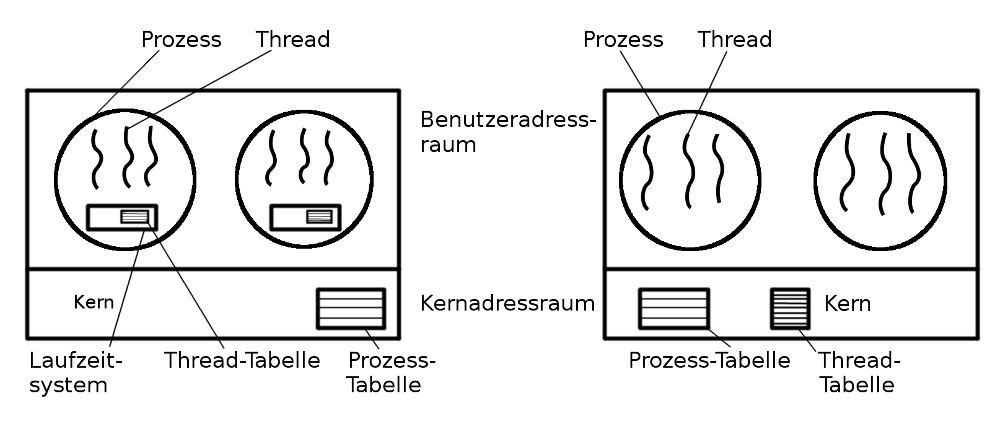
\includegraphics[scale=1.2]{kernelthreads.jpg}\\
\subsubsection{Implementierung von Threads im Benutzeradressraum}
Wenn Threads in der \textbf{Anwenderebene} laufen, braucht jeder Threads seine eigene private Thread-Tabelle. Wenn ein Thread seinen Zustand wechselt, dann werden alle Infomationen die gebraucht werden, in der Thread-Tabelle gespeichert.\\
Wenn ein Thread etwas tut, was ihn \textbf{lokal blockieren} könnte, zB wenn er auf einen anderen Thread wartet, dann ruft er eine Funktion des \textbf{Laufzeitsystems} auf. Muss der Thread blockiert werden, so speichert dieser die Register des Threads in der Thread-Tabelle, sucht in dieser Tabelle einen rechenbereiten Thread und startet diesen. Ein solcher Thread-Wechsel im Anwendermodus ist \textbf{deutlich schneller} als ein Sprung in den Kern.\\
Thread-Pakete auf Benutzerebene haben trotz besserer Performance schwerwiegende Probleme. Das erste ist das Problem mit den \textbf{blockierenden Systemaufrufen}. Ein Thread kann nicht einfach einen Systemaufruf machen, dies würde den gesamten Prozess blockieren, was gegen den Sinn von Threads geht. Man könnte also die blockierenden Aufrufe wie \textbf{read} durch eine neue, nicht blockierende Version ersetzen. \\
Ähnlich ist das Problem der Seitenfehler. Wenn ein das Programm einen Befehl aufruft, der nicht im Cache ist, muss er diesen von der Platte holen. Das wird als \textbf{page fault} bezeichnet.\\
Außerdem können die anderen Threads nicht arbeiten, bis der erste Thread freiwillig die CPU freigibt, da es innerhalb eines Prozesses keine \textbf{Timerinterrupts} gibt. Dies muss also ineffizient und grob "manuell" gehandhabt werden.\\
Meistens sind Threads in Anwendungen gewünscht, die oft Systemaufrufe ausführen und somit blockieren. Man möchte eine bessere Effizienz indem ständig zwischen Threads umgeschaltet werden kann, sobald ein anderer blockiert.\\
\subsubsection{Implementierung von Threads im Kern}
Wenn Threads im Kern laufen und der Kern also die Threads kennt, wird kein \textbf{Laufzeitsystem} benötigt. Jede Erzeugung oder Zerstörung von Threads wird von einem Kernaufruf durchgeführt. Die Thread-Tabelle im Kern enthält Register, Zustand und andere Informationen zu jedem Thread.\\
Alle Aufrufe, die einen Thread blockieren könnten, sind als Systemaufrufe realisiert und verursachen dadurch weit höhere Kosten als ein Prozeduraufruf im Laufzeitsystem. Wenn ein Thread blockiert wird, ist aber \textbf{nicht} der gesamte Prozess blockiert. Der Kern hat nun die Wahl einen Thread aus dem gleichen Prozess anzusprechen oder einen anderen Prozess rechnen zu lassen.\\
Da das Erzeugen und Zerstören von Threads so kostenaufwändig ist, werden die Threads meist \textbf{recycled}. Ein Thread wird also nicht wirklich zerstört, sondern als nicht lauffähig gekennzeichnet. Dabei behält er seine Datenstrukturen im Kern und kann wiederverwendet werden. \\
Threads im Kernmodus erfordern keine neuen, nicht blockierenden Systemaufrufe. Hauptnachteil der Kern-Threads sind die deutlich höheren Kosten eines Systemaufrufs.\\
Das Problem beim fork eines Prozesses mit mehreren Threads besteht jedoch weiterhin. Sollte ein Kindprozess die Anzahl der Threads erben oder nicht. Was sinnvoller ist, kommt auf den Kontext an. Soll ein neues Programm vom Kindprozess aufgerufen werden, sollte der Kindprozess besser nur einen Thread besitzen. Soll er mit der Ausführung fortfahren, sollte er besser die Threads erben.
\subsubsection{Hybride Implementierungen}
Um die Vorteile von Benutzer-Threads und Kern-Threads zu verbinden wurden verschiedene Möglichkeiten untersucht. Einer ist die Verwendung von Kern-Threads in welchen dann Benutzer-Threads ablaufen. \\
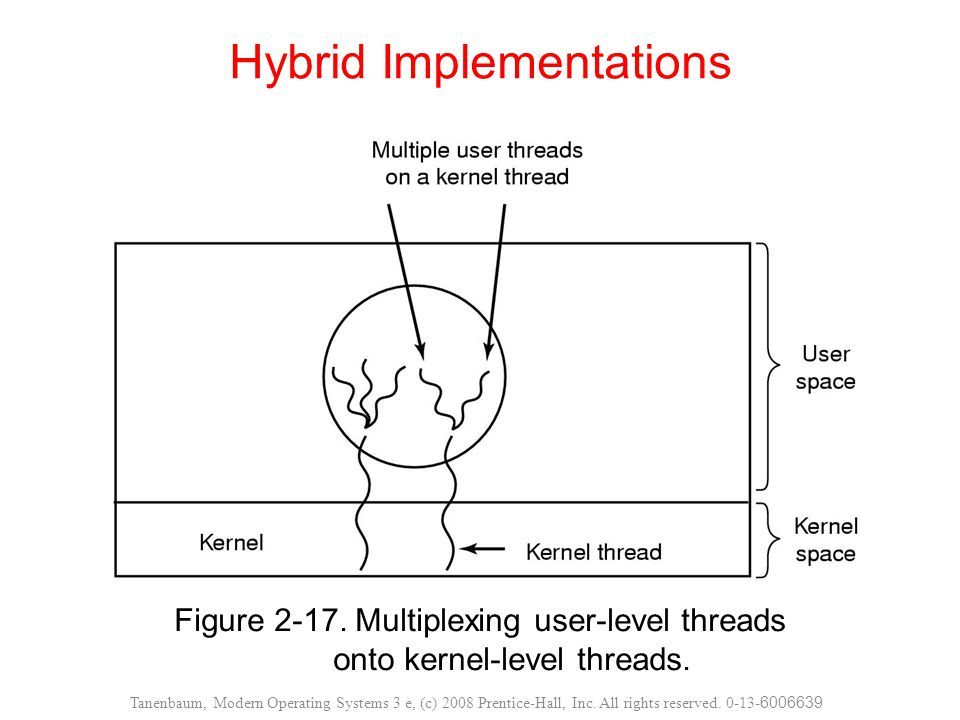
\includegraphics[scale=0.5]{hybridthreads.jpg}\\
Bei dieser Vorgehensweise ist dich der Kerb \textit{nur} der Kern-Threads bewusst. Manche dieser Threads haben dann mehrere Benutzer-Threads die auf ihnen gebündelt sind.
\subsubsection{Scheduler-Akitivitäten}
Eine andere Art um die Vorteile von Benutzer-Threads und Kern-Threads zu verbinden. Der Ansatz, der hier beschrieben wird, heit \textbf{Scheduler-Aktivierungen}.\\
Das Ziel von Scheduler-Aktivierungen ist folgendes zu verbinden: 
\begin{itemize}
\item{bessere Performanz als Kern-Threads}
\item{größere Flexibilität, wie Benutzerraum-Threads}
\item{keine Notwendigkeit für spezielle, nicht blockierende Systemaufrufe}
\item{Wenn ein Thread blockiert ist, soll nicht der gesamte Prozess blockiert werden}
\end{itemize}
\textbf{Effizenz} soll dadurch erreicht werden, dass es keine unnötige Wechsel zwischen Benutzer- und Kernadressraum gibt. Wenn das Laufzeitsystem den Prozess blockieren kann, so sollte es das auch tun und nicht in den Kernmodus umschalten.\\
Um es zu schaffen, dass nicht alle Threads auf einmal durch einen Hardwareinterrupt blockiert werden, werden bei Scheduler-Aktivierungen dem Prozess \textbf{mehrere virtuelle Prozessoren} zugeordnet.\\
Auf diesen virtuellen Prozessoren laufen Kern-Threads auf denen wiederrum Benutzerraum-Threads laufen.\\
Wenn der Kern weiß, dass ein Thread blockiert hat (also ein Kern-Thread), dann informiert er mit einem \textbf{Upcall} das Laufzeitsystem. Daraufhin teilt das Laufzeitsystem seine Threads neu ein, markiert also diesen Thread als blockiert und wählt einen anderen rechenbereiten Thread aus.\\\\
Bei einem Hardware-Interrupt während ein Benutzerraum-Thread läuft, wechselt die unterbrochene CPU in den Kernmodus.???? Morgen weiter durchlesen

\subsection{Interprozesskommunikation}
\subsection{Scheduling}
\subsection{Klassische Probleme der Interprozesskommunikation}
\subsection{Forschung zu Prozessen und Threads}
\subsection{Aufgaben}
\end{document}